
\documentclass[a4paper,14pt]{extarticle}

\usepackage[utf8]{inputenc}
\usepackage[T1]{fontenc}
\usepackage[english,russian]{babel}
\usepackage[oglav,spisok,boldsect,eqwhole,figwhole,hyperref,hyperprint,remarks,greekit]{./style/fn2dipstyle_Sveta}
\graphicspath{{./style/}{./figures/}}

\usepackage{setspace}
\setstretch{1.5}
\usepackage[left=3cm,right=1cm, top=2cm,bottom=2cm]{geometry}
\usepackage{pdfpages}
\pagestyle{plain}
\usepackage{mathtools}

% Центрированные таблицы фиксированной ширины %
\usepackage{tabularx} % also loads 'array' package
\newcolumntype{C}{>{\centering\arraybackslash}X} % centered version of 'X' columns

\usepackage{relsize}
\newcommand{\smallalpha}{\mathsmaller{(} \alpha \mathsmaller{)}}
\newcommand{\smallbeta}{\mathsmaller{(} \beta \mathsmaller{)}}
\newcommand{\avg}[1]{\left\langle #1 \right\rangle}
\usepackage[titles]{tocloft}

\usepackage{multirow}
\usepackage{supertabular}
\usepackage{multicol}
\usepackage{amsmath}
\usepackage{afterpage}
\usepackage{amsmath}
% Параметры титульного листа
%\title{Решение уравнения Рейнольдса\\ в рамках теории газовой смазки \\ методом конечных элементов}
%\author{В.\,Г.~Пиневич}
%\supervisor{А.\,В.~Селиванов}
%\group{ФН2-81Б}
%\date{2024}

% Переопределение команды \vec, чтобы векторы печатались полужирным курсивом
\renewcommand{\vec}[1]{\text{\mathversion{bold}${#1}$}}%{\bi{#1}}
\newcommand\thh[1]{\text{\mathversion{bold}${#1}$}}
%Переопределение команды нумерации перечней: точки заменяются на скобки
\renewcommand{\labelenumi}{\theenumi)}
\begin{document}
	
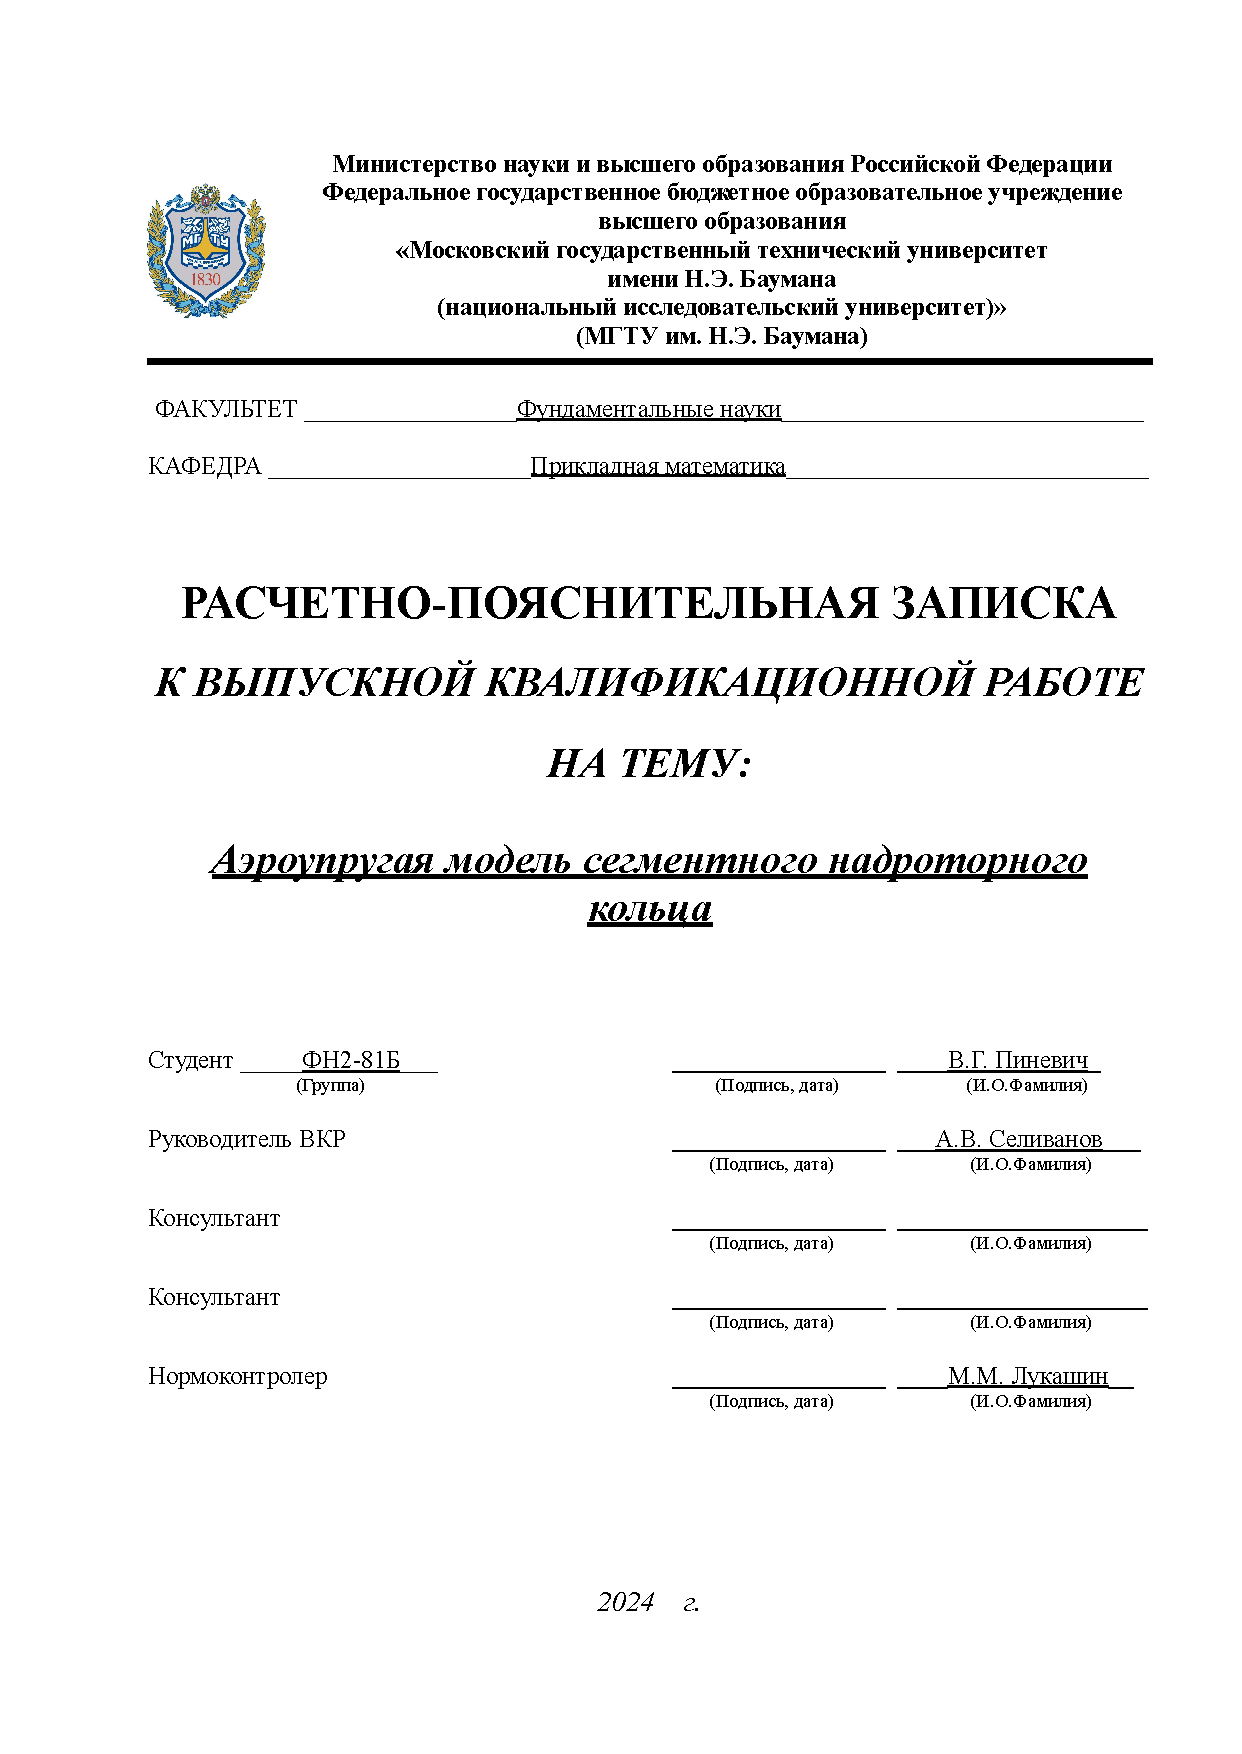
\includepdf[pages=1]{filled-title.pdf}
	
%\section-{\large{РЕФЕРАТ}}	
\section-{\large{Реферат}}	

Расчетно-пояснительная записка 41 с., 24 рис., 3 табл., 8 источников, 1
прил.

МЕТОД КОНЕЧНЫХ ЭЛЕМЕНТОВ, УРАВНЕНИЕ РЕЙНОЛЬДСА,
АЭРОУПРУГАЯ МОДЕЛЬ.

Составлено решение уравнение Рейнольдса методом конечных элементов. Решение может быть получено как для переменной, так и для постоянной правой части. 

Численные результаты, полученные с помощью разработанной программы были проверены с помощью подстановки правой части, полученной от заведомо известной функции, в модель, а также сравнены со результатами вычисления функции NSolve Wolfram Mathematica.

Получены решения задачи Рейнольдса для различных наклонов зазора и граничных условий, проведено их сравнение.

Модель решения уравнения Рейнольдса была дополнена с помощью ограничения движения пластины пружиной сверху. Найдено положение равновесия, проверена устойчивость этого положения.

\newpage

\tableofcontents

\newpage

%\section-{\large{ВВЕДЕНИЕ}}
\section-{\large{Введение}}
Задачи расчёта подшипников газодинамического типа с зазорами разнообразной формы до сих пор остаются весьма актуальными. По сути, они сводятся к изучению газового смазочного слоя в тонком зазоре произвольной формы. Решением таких задач занимается гидродинамическая теория смазки. Этот раздел механики жидкости и газа начал развиваться в конце XIX века вслед за потребностями техники. Начало теоретическому исследованию течений в тонких зазорах положили работы Н. П. Петрова и британского учёного Осборна Рейнольдса, уточнённые и доведённые до возможности практического применения А. Зоммерфельдом, А. Мичелем. Дальнейшие исследования позволили распространить результаты созданной Рейнольдсом теории на газодинамические подшипники. Были даже предприняты успешные попытки получения общего вида уравнения Рейнольдса для смазочного слоя без привязки к конкретной системе координат. 

Николай Павлович Петров --- русский учёный-механик и инженер, инженер-генерал, профессор, основоположник гидродинамической теории смазки. В 1883 году в «Инженерном журнале» издаётся первая работа Н. П. Петрова по гидродинамической теории смазки «Трение в машинах и влияние на него смазывающих масел». За её создание в 1884 году он стал лауреатом Ломоносовской премии. В 1886 году была опубликована вторая работа — «Описание и результаты опытов над трением жидкостей и машин»; а в 1887 году — третья книга — «Трение в машинах и влияние на него смазывающей жидкости. Практические результаты опытов». В 1900 году в «Записках» Академии наук вышло в свет четвёртое крупное сочинение Н. П. Петрова — «Трение в машинах», в котором изложена теория смазки с учётом эксцентрического положения шипа в подшипнике. За свою жизнь опубликовал более 80 научных работ и был удостоен многих премий.

\newpage

Осборн Рейнольдс ---  английский механик, физик и инженер, специалист в области гидромеханики и гидравлики, член Лондонского королевского общества. Экспериментально установил критерий перехода ламинарного режима движения жидкости, текущей в цилиндрической трубе, в турбулентный режим; данный критерий заключается в том, что введённая Рейнольдсом безразмерная величина (названная в его честь числом Рейнольдса) превышает некоторое критическое значение. Применительно к турбулентному движению вывел дифференциальные уравнения осреднённого движения жидкости, содержащие нерегулярные пульсационные добавки. Сформулировал критерий подобия двух различных течений вязкой жидкости.
В 1886 году учёный развил гидродинамическую теорию смазки; при этом предложил дифференциальное уравнение, характеризующее распределение давления в вязкой жидкости, которая заполняет собой зазор между поверхностями вала и подшипника.
Исследовал явления кавитации, групповой скорости распространения волн на свободной поверхности жидкости, теплопередачи от стенок сосуда к жидкости. Определил механический эквивалент теплоты.
Рейнольдс был первым, кто исследовал природу трения качения упругих катков по упругим основаниям; в своей работе 1876 года он изучал качение резиновых и стальных катков по резиновым и стальным плоским основаниям. Причину возникновения трения качения он видел во взаимном частичном проскальзывании поверхностей катка и основания.

Для извлечения из решения уравнения Рейнольдса практической пользы можно добавить ограничение движения верхней стенки пружиной и таким образом получить динамическую систему. Для описания подобных динамических систем используются уравнения Лагранжа.

Жозееф Луи Лагранж --- французский математик, астроном и механик итальянского происхождения. Наряду с Эйлером -- крупнейший математик XVIII века. Особенно прославился исключительным мастерством в области обобщения и синтеза накопленного научного материала. Одним из наиболее известных достижений Лагранжа является его теория аналитической механики, которая включает формулирование принципа наименьшего действия и разработку общей теории вариационного исчисления.  Лагранж сделал значительный вклад в область математического анализа, в том числе в теорию функций и дифференциальных уравнений. Его работы о функциональном анализе стали основой для развития этой области математики. Лагранж разработал методы решения разнообразных задач физики, включая задачи о движении небесных тел и механике деформируемых тел.Его труды по теории чисел имеют большое значение для математики, в частности, он ввел понятие символа Лежандра и занимался исследованием квадратичных форм. Лагранж также внес вклад в область оптики, изучая световые явления и разрабатывая методы анализа оптических систем. Его работы по алгебре и теории уравнений были значимыми для развития алгебраической геометрии и групповой теории.

\section-{Постановка задачи}

Для создания газотурбинного двигателя в настоящее время требуется уплотнение зазоров во многих элементах конструкции~\cite{sel-1}. Это необходимо для улучшения характеристик двигателя и его надежности. Уплотнители разделяют на контактные и бесконтактные. Они имеют понятные преимущества и недостатки по сравнению друг с другом. По скольку трение много выше при использовании контактного уплотнителя, это приводит к его более быстрому износу, однако позволяет создать постоянный контакт с уплотняемой деталью и получить лучшую эффективность. С другой стороны, бесконтактный уплотнитель более долговечен, но уровень утечек при их использовании выше. Для расчета уплотнений также используются математическое моделирование.

По данным NASA, использование в современных двигателях перспективных уплотнений позволит уменьшить удельный расход топлива на 2–3\%~\cite{nasa}. Одной из наиболее перспективных разработок в этой области являются
пальчиковые уплотнении.
\begin{figure}[!htbp]
	\center{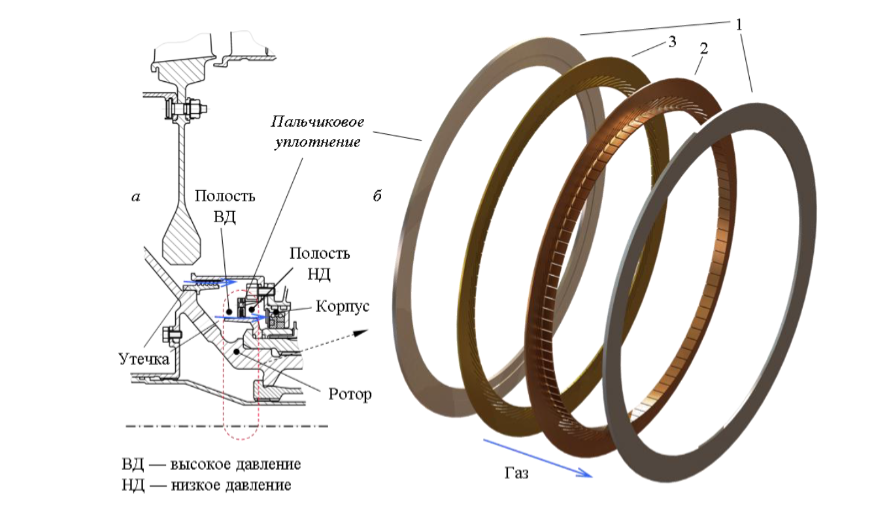
\includegraphics[width=\textwidth, height=0.5\textwidth]{vved-1.png}}
	\caption{Конструкция и схема балансировки бесконтактного пальчикового
		уплотнения: 1 — корпус уплотнения; 2 — передняя пластина с пальчиками;
		3 — ротор; 4 — задняя пластина с пальчиками и подъемными площадками}
	\label{vved-1}
\end{figure}
Пальчиковые уплотнители состоят из множества гибких элементов. Они представляют собой сборку из двух тонких соосных уплотняющих кольцевых пластин с прорезями и двух утолщенных сплошных корпусных дисков, закрепленных вместе по внешнему диаметру заклепкам~(рис.~\ref{vved-1}).

Были предложены различные методы для увеличения эффективности
использования пальчиковых уплотнений. Например, выполнение небольшой
площадки вытянутой в осевом направлении на конце каждого пальца для
снижения износа~(рис.~\ref{vved-2})
\begin{figure}[!htbp]
	\center{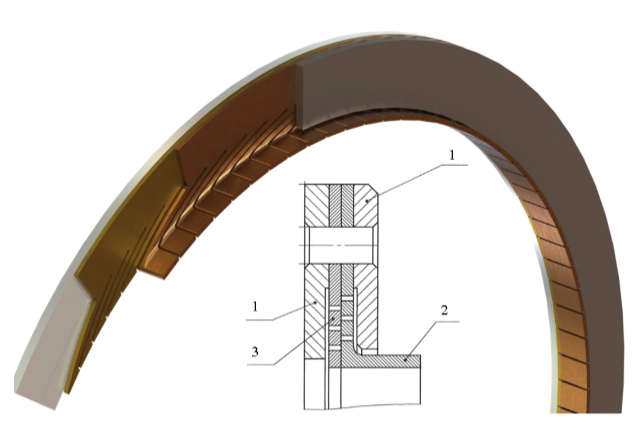
\includegraphics[width=\textwidth, height=0.5\textwidth]{vved-2.png}}
	\caption{Схема бесконтактного пальчикового уплотнения: 1 – корпусные
		диски; 2 и 3 – задняя и передняя уплотняющие пластины}
	\label{vved-2}
\end{figure}

Ключевым моментом в обеспечении работоспособности бесконтактного пальчикового уплотнения является балансировка пальчиков в потоке газа.
Принцип этой балансировки основан на возникновении сил газостатического и газодинамического давления в зазоре под площадками, которые уравновешивают силы реакции при деформировании пальчиков и силы внешнего
давления, действующие на уплотнение со стороны газа в полости. При увеличении радиуса ротора зазор под площадками уменьшается, что ведет к
увеличению подъемной силы и, соответственно, к перемещению пальчиков в
направлении от ротора. Наступление баланса сил определяет новое положение площадок и рабочий зазор.

\begin{figure}[!htbp]
	\center{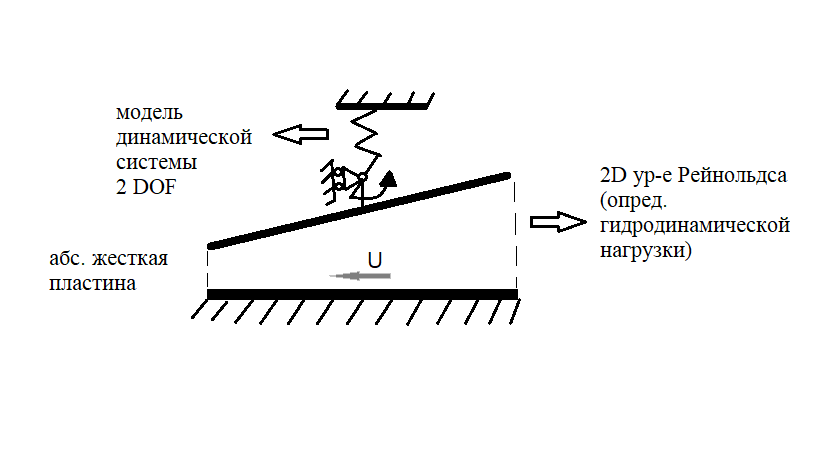
\includegraphics[width=\textwidth, height=0.55\textwidth]{pruzina-text.png}}
	\caption{Схема бесконтактного пальчикового уплотнения: 1 – корпусные
		диски; 2 и 3 – задняя и передняя уплотняющие пластины}
	\label{pruzina-text}
\end{figure}
В данной работе будут решаться следующие задачи:
	\begin{enumerate}	
	\item Построить модель для исследования положения равновесия сегментов надроторного кольца в потоке жидкости.
	\item Исследовать на устойчивость найденное положение равновесия.
\end{enumerate}

\section{Решения уравнения Рейнольдса}

Задача данной главы --- вывести, а затем  решить дифференциальное уравнения Рейнольдса методом конечных элементов.
\begin{equation}
	\label{reinolts-task}
	\frac{\partial}{\partial x} \left(h^3 \frac{\partial p}{\partial x} \right) + \frac{\partial}{\partial z} \left(h^3 \frac{\partial p}{\partial z} \right) = 6 \mu U \frac{\partial h}{\partial x} \text{, }
\end{equation}
где $h = h(x)$ --- толщина слоя, $p = p(x, z)$ --- давление, $\mu$ --- коэффициент вязкости. Граничные условия: $U$ --- скорость в направлении $x$ на одной из пластин, $p_{\text{в}}$ --- повышенное давление, $p_{\text{н}}$ --- пониженное давление. 

Размеры области зададим 5 мм по ширине и 5 мм по длине. Будем использовать коэффициент вязкости воды $\mu = 8.90 \cdot 10^{-4} \text{ Па} \cdot \text{с}$.
\newline Давление возьмем $p_{\text{н}} = 100 \text{ кПа}, p_{\text{в}} = 150 \text{ кПа}$. Скорость будет меняться в зависимости от специфики расчетов. Схематичное изображение области задачи и граничных условий изображено на рис.~\ref{obl_resh}.

\begin{figure}[!htbp]
	\center{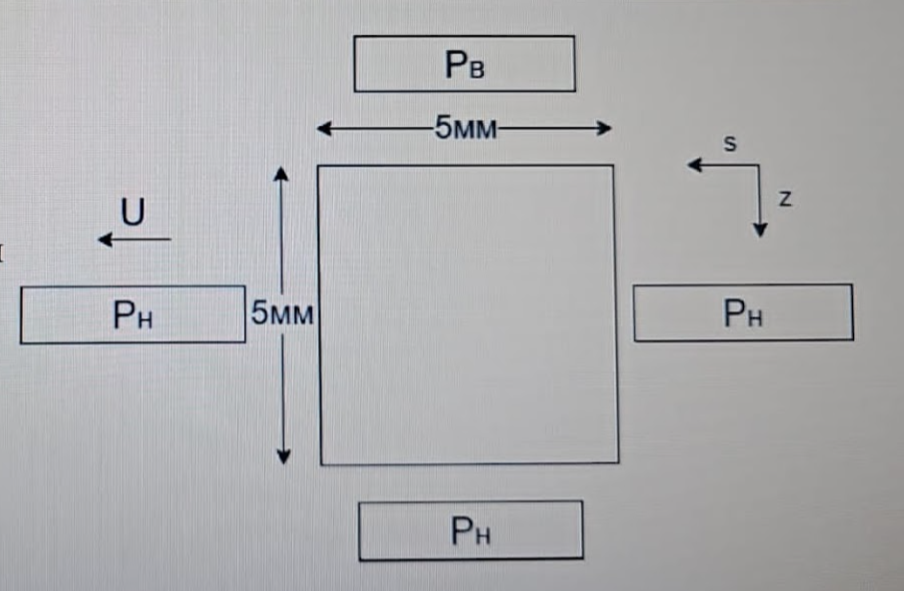
\includegraphics[width=\textwidth, height=0.5\textwidth]{taskGU.png}}
	\caption{Схема области решения и граничных условий уравнения Рейнольдса}
	\label{obl_resh}
\end{figure}

\subsection{Получение уравнения Рейнольдса}

Уравнение Рейнольдса является одним из основных уравнений в области механики жидкостей и газов. Оно было названо в честь физика Осгуда Рейнольдса, который впервые сформулировал его в середине XIX века.
Уравнение Рейнольдса имеет широкое применение в различных областях науки и техники, таких как гидродинамика, аэродинамика, теплообмен. Это уравнение является основой для предсказания и анализа различных явлений, связанных с течением жидкостей и газов.
Гидродинамические уравнения несжимаемой жидкости с
внутренним трением могут быть представлены в очень простой
форме, если пренебречь силами, пропорциональными массам,
равно как и силами инерции.

Рассмотрим получение уравнения Рейнольдса из~\cite{petrov_smazka}. Обозначая через $x$, $y$, $z$ прямоугольные координаты точки, через $p$ -- гидродинамическое давление в этой точке,

Силы трения $p_{xy}, p_{xz}, p_{yx}, p_{yz}, p_{zx}, p_{zy}$, перпендикулярные к оси силы, обозначенной первой буквой индекса и параллельные оси силы, обозначенной второй буквой индекса.

Обозначим проекции скорости на осях $x, y, z \text{ соответственно}$ $u, \nu, \omega$.

Введем $\mu$ как коэффициент внутреннего трения жидкости.ы
Тогда можно записать три системы уравнений:
\begin{enumerate}
	\item Система, определяющая гидродинамическое давление в
	точках $x, y, z$:
	\begin{equation}
		\label{eqfi}
		\begin{cases}
			\frac{\partial p}{\partial x} = \mu \left( \frac{\partial^2 u}{\partial x^2} + \frac{\partial^2 u}{\partial y^2} + \frac{\partial^2 u}{\partial z^2} \right), \\
			\frac{\partial p}{\partial y} = \mu \left( \frac{\partial^2 \nu}{\partial x^2} + \frac{\partial^2 \nu}{\partial y^2} + \frac{\partial^2 \nu}{\partial z^2} \right), \\
			\frac{\partial p}{\partial z} = \mu \left( \frac{\partial^2 \omega}{\partial x^2} + \frac{\partial^2 \omega}{\partial y^2} + \frac{\partial^2 \omega}{\partial z^2} \right).
		\end{cases}
	\end{equation}
	\item Система, определяющая силы трения в той же точке:
	\begin{equation}
		\label{eqsi}
		\begin{cases}
			p_{yz} = p_{zy} = \mu \left(\frac{\partial \omega}{\partial y} + \frac{\partial \nu}{\partial z} \right), \\
			p_{zx} = p_{xz} = \mu \left( \frac{\partial \omega}{\partial x} +  \frac{\partial u}{\partial z} \right), \\
			p_{xy} = p_{yx} = \mu \left(  \frac{\partial u}{\partial y} + \frac{\partial \nu}{\partial x} \right).
		\end{cases}
	\end{equation}
	\item Условие несжимаемости жидкости, выраженное уравнением: 
	\begin{equation}
		\label{eqthi}
		\frac{\partial u}{\partial x} + \frac{\partial \nu}{\partial y} + \frac{\partial \omega}{\partial z} = 0.
	\end{equation}
	
\end{enumerate}

Примем, что скорость $\nu = 0$, поскольку она мала по сравнению со скоростями $u = 0$, $\omega = 0$.

Изменения скоростей $u$ и $\omega$ со при заданном значении $y$ для всех изменений $ x $ и $z$ могут рассматриваться как чрезмерно малые, поэтому примем
\[
\frac{\partial^2 u}{\partial x^2} = 0, 
\frac{\partial^2 u}{\partial z^2} = 0, 
\frac{\partial^2 \omega}{\partial x^2} = 0, 
\frac{\partial^2 \omega}{\partial z^2} = 0. 
\]

Ограничиваясь приближенным решением, которое можно
получить при указанных выше предположениях, уравнения \eqref{eqfi}, \eqref{eqsi} и \eqref{eqthi} могут быть приведены к следующей форме.
\begin{equation}
	\label{secondinitialeq}
	\begin{cases}
		\frac{\partial p }{\partial x} = \mu \frac{\partial^2 u}{\partial y^2}, \\
		\frac{\partial p }{\partial y} = 0, \\
		\frac{\partial p }{\partial z} = \mu \frac{\partial^2 \omega}{\partial y^2}.
	\end{cases}
\end{equation}
\begin{equation}
	\label{secinitialeq}
	\begin{cases}
		p_{yz} = p_{xy} = \mu \frac{\partial \omega}{\partial y}, \\
		p_{zx} = p_{xz} = 0, \\
		p_{xy} = p_{yx} = \mu \frac{\partial u}{\partial y}.
	\end{cases}
\end{equation}
\begin{equation*}
	\frac{\partial u}{\partial x} + \frac{\partial \nu}{\partial y} + \frac{\partial \omega}{\partial z} = 0.
\end{equation*}

Для определения давления необходимо интегрировать выражения \eqref{secondinitialeq}, \eqref{secinitialeq}. Для этого определим граничные условия.

\noindent Для $y = 0$ имеем
\[
\begin{cases}
	u = U_0, \\
	\nu = 0, \\
	\omega = 0.
\end{cases}
\]

\noindent Для $y = h$ имеем
\[
\begin{cases}
	u = U_1, \\ 
	\nu = U_1 - U_1 \frac{\partial  h}{\partial h}, \\ \omega = 0.
\end{cases}
\]

Поскольку $p$ не зависит от $y$, то интегрирование уравнений \eqref{secondinitialeq} приводит к уравнениям
\begin{equation}
	\label{1-inte-inti}
	\begin{cases}
		u = \frac{1}{2 \mu} \frac{\partial p}{\partial x} \left( y - h \right) y + U_0 \frac{h - y}{h} + U_1 \frac{y}{h},\\
		\omega = \frac{1}{2 \mu} \frac{\partial p}{\partial z} (y - h) y.
	\end{cases}
\end{equation} 
Первые производные вторых членов этих уравнений, перенесенные в соответствующие уравнения группы \eqref{secinitialeq}, приводят
к уравнениям
\begin{equation}
	\label{sec-init-eq}
	\begin{cases}
		p_{yz} = p_{zy} = \frac{1}{2} \frac{\partial p}{\partial z} \left( 2y - h \right), \\
		p_{xy} = p_{yz} = \frac{1}{2} \frac{\partial p}{\partial x} \left( 2y - h \right) + \mu \frac{U_1 - U_0}{h}.
	\end{cases}
\end{equation}

Если давление $p$ считать независимым от координаты $z$, то четыре последних
уравнения сокращаются до двух: первое из системы~\eqref{1-inte-inti} и
второе из системы~\eqref{sec-init-eq}.

Взяв производные от первого из этих уравнений по $x$ и
от второго по $z$ и подставляя это в уравнение~\eqref{eqthi}, находим, что
\begin{equation*}
	\frac{\partial \nu}{\partial y} = - \frac{1}{2 \mu} \left( \frac{\partial}{\partial x} \left( \frac{\partial p}{\partial x} (y - x) y \right) + \frac{\partial}{\partial z} \left( \frac{\partial p}{\partial z} (y - h) h \right) - \frac{\partial}{\partial x} \left( U_0 \frac{h - y}{h} + U_1 \frac{y}{h} \right) \right).
\end{equation*}

Интегрируя это уравнение в пределах от $y = 0$ до $y = h$ и
принимая во внимание граничные условия, получаем
\begin{equation*}
	\frac{\partial}{\partial x} \left( h^3 \frac{\partial p}{\partial x} \right) + \frac{\partial}{\partial z} \left( h^3 \frac{\partial p}{\partial z} \right) = 6 \mu \left( (U_0 - U_1) \frac{\partial h}{\partial x} \right) + 2 V_1.
\end{equation*}
$2 V_1$ используется для учёта движений одной из стенок зазора, меняющих значение функции. Если пренебречь этим, и обозначить $U_0 - U_1$ как $U$, то получим искомое уравнение~\eqref{reinolts-task}.

Решение уравнения Рейнольдса~\eqref{reinolts-task} будем искать с помощью метода конченых элементов.
Метод конечных элементов (МКЭ) является одним из самых мощных инструментов инженерного анализа конструкций и материалов. Его история восходит к 1940-м годам, когда инженеры начали использовать численные методы для решения сложных инженерных задач. Однако истоки метода конечных элементов можно проследить еще в XIX веке, когда математики и физики начали разрабатывать методы для решения дифференциальных уравнений. 
Существенный толчок в своём развитии метода конечных элементов получил в 1963 году после того, как было доказано, что его можно рассматривать как один из вариантов распространённого в строительной механике метода Рэлея-Ритца, который путём минимизации потенциальной энергии сводит задачу к системе линейных уравнений равновесия. Область применения метода конечных элементов значительно расширилась, когда было установлено, что уравнения, определяющие элементы в задачах, могут быть легко получены с помощью вариантов метода взвешенных невязок, таких как метод Галеркина или метод наименьших квадратов. Это сыграло важную роль в теоретическом обосновании метода конечных элементов, так как позволило применять его при решении многих типов дифференциальных уравнений. Таким образом, метод конечных элементов превратился в общий метод численного решения дифференциальных уравнений или систем дифференциальных уравнений. Первые приложения МКЭ к инженерным задачам появились во второй половине XX века, когда компьютеры стали доступны для широкого круга специалистов. С появлением компьютерных программ, способных решать большие системы уравнений, МКЭ стал неотъемлемой частью инженерного проектирования.
Основная идея метода конечных элементов состоит в том, что любую непрерывную величину, такую как температура, давление и перемещение, можно аппроксимировать дискретной моделью, которая строится на множестве кусочно-непрерывных функций, определенных на конечном числе подобластей. Кусочно-непрерывные функции определяются с помощью значений непрерывной величины в конечном числе точек рассматриваемой области.
В общем случае непрерывная величина заранее неизвестна и нужно определить значения этой величины в некоторых внутренних точках области. Дискретную модель, однако, не сложно построить, если сначала предположить, что числовые значения этой величины в каждой внутренней точке области известны. После этого можно перейти к общему случаю. Итак, при построении дискретной модели непрерывной величины поступают следующим образом:
\begin{enumerate}
	\item В рассматриваемой области фиксируется конечное число точек. Эти точки называются узловыми точками или просто узлами.
	\item Значение непрерывной величины в каждой узловой точке считается переменной, которая должна быть определена.
	\item Область определения непрерывной величины разбивается на конечное число подобластей, называемых элементами. Эти элементы имеют общие узловые точки и в совокупности аппроксимируют форму области.
	\item Выбор функций формы и аппрокисмирующей функции.
	\item Построение локальной матрицы.
	\item Построение глобальной матрицы путем сшивания локальных матриц элементов друг с другом.
	\item Учет граничных условий путем заменой коэффициентов в полученной матрице или же вектора правых частей.
	\item Решение системы линейных уравнений для получения решения в узловых точках.
\end{enumerate}

\subsection{Метода Галеркина}

Существуют разные подходы к реализации идеи метода конечных элементов. В данной работе рассмотрим методику решения с помощью метода Галеркина. Для разбиения области на элементы требуется выбрать форму элемента. Поскольку рассматриваемая область прямоугольная, то удобно взять элементы прямоугольной формы. 

\begin{figure}[!htbp]
	\center{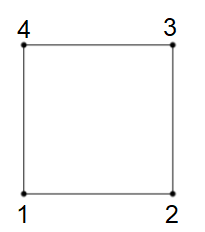
\includegraphics[width=0.3\textwidth, height=0.3\textwidth]{base_element.png}}
	\caption{Линейный прямоугольный конечный элемент}
	\label{base_element}
\end{figure}
\begin{figure}[!htbp]
	\center{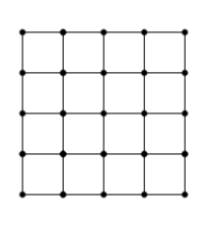
\includegraphics[width=0.3\textwidth, height=0.3\textwidth]{base_element_proection.png}}
	\caption{Проекция расчётной области}
	\label{base_element_proection}
\end{figure}

Пусть $l$ --- горизонтальная длинная области, а $h$ --- вертикальная. Тогда функции формы будут иметь следующий вид~\cite{seshu}:
\begin{equation}
	\begin{cases}
		N_1 = 1 - \frac{x}{l} - \frac{z}{h} + \frac{x  z}{l  h}, \\
		N_2 = \frac{x}{l} - \frac{x  z}{l  h}, \\
		N_3 = \frac{x  z}{l h}, \\
		N_4 = \frac{z}{h} - \frac{x  z}{l  h}. \\
	\end{cases}
\label{form-func}
\end{equation}

\noindent
Аппроксимирующую функцию зададим в виде:
\begin{equation*}
	\phi = c_0 N_1 + c_1 N_2 + c_2 N_3 + c_3 N_4.
\end{equation*}
\noindent 
Обратимся к источнику~\cite{slezkin_smazka}. Далее будем искать локальную матрицу из выражения:
\begin{equation}
	\label{init_eq}
	\int_{S_i} {[N]^T \left(\frac{\partial}{\partial x} \left(h^3 \frac{\partial p}{\partial x} \right) + \frac{\partial}{\partial z} \left(h^3 \frac{\partial p}{\partial z} \right) - 6 \mu U \frac{\partial h}{\partial x}\right) dx dz} = 0.
\end{equation}
$S_i$ --- область, содержащая элемент. 
Подставим аппрокисимирующую функцию $\phi$ вместо $p$.
\begin{equation*}
	\int_{S_i} {[N]^T \left(\frac{\partial}{\partial x} \left(h^3 \frac{\partial \phi}{\partial x} \right) + \frac{\partial}{\partial z} \left(h^3 \frac{\partial \phi}{\partial z} \right) - 6 \mu U \frac{\partial h}{\partial x}\right) dx dz} = 0.
\end{equation*}
Понизим порядок производной с помощью функции дифференцирования произведения:
\begin{equation*}
	 \frac{\partial}{\partial x} \left( [N]^T h^3 \frac{\partial \phi}{\partial x} \right)  = [N]^T \frac{\partial}{\partial x} \left(h^3 \frac{\partial \phi}{\partial x} \right) + \frac{\partial[N]^T}{\partial x} \left(h^3 \frac{\partial \phi}{\partial x} \right),
\end{equation*}
\begin{equation*}
	 \frac{\partial}{\partial z} \left( [N]^T h^3 \frac{\partial \phi}{\partial z} \right)  = [N]^T \frac{\partial}{\partial z} \left(h^3 \frac{\partial \phi}{\partial z} \right) + \frac{\partial[N]^T}{\partial z} \left(h^3 \frac{\partial \phi}{\partial z} \right).
\end{equation*}

Подставим полученные выражения в исходный интеграл~\eqref{init_eq}:
\begin{equation*}
\int_{S_i} {\left(\frac{\partial}{\partial x} \left( [N]^T h^3 \frac{\partial \phi}{\partial x} \right) - \frac{\partial[N]^T}{\partial x} \left(h^3 \frac{\partial \phi}{\partial x} \right) \right) dxdz} + 
\end{equation*}
\begin{equation*}
 + \int_{S_i} {\left(\frac{\partial}{\partial z} \left( [N]^T h^3 \frac{\partial \phi}{\partial z} \right) - \frac{\partial[N]^T}{\partial z} \left(h^3 \frac{\partial \phi}{\partial z} \right) - [N]^T 6 \mu U \frac{\partial h}{\partial x}\right) dxdz} = 0.
\end{equation*}

С помощью формулы Грина можно заменить третье и первое слагаемое под знаком интеграла~\cite{seligard}:
\begin{equation*}
	\int_{S_i} {\left(\frac{\partial}{\partial x} \left( [N]^T h^3 \frac{\partial \phi}{\partial x} \right) + \frac{\partial}{\partial z} \left( [N]^T h^3 \frac{\partial \phi}{\partial z} \right)  \right)   dxdz} =
\end{equation*}
\begin{equation*}
	= \oint_{\partial S_i} { \left( [N]^T h^3 \frac{\partial \phi}{\partial x} l_x +   [N]^T h^3 \frac{\partial \phi}{\partial z} l_z \right)  d \left( \partial S_i \right)}.
\end{equation*}

Выражение~\eqref{init_eq} примет вид:
\begin{equation*}
	\oint_{\partial S_i} { \left( [N]^T h^3 \frac{\partial \phi}{\partial x} l_x +   [N]^T h^3 \frac{\partial \phi}{\partial z} l_z \right)  d \left( \partial S_i \right)} -
\end{equation*}
\begin{equation*}
	- \int_{S_i} {\left( \frac{\partial[N]^T}{\partial x} \left(h^3 \frac{\partial \phi}{\partial x} \right) +  \frac{\partial[N]^T}{\partial z} \left(h^3 \frac{\partial \phi}{\partial z} \right) - [N]^T 6 \mu U \frac{\partial h}{\partial x}\right) dxdz} = 0.
\end{equation*}

Поскольку в условии задачи заданы граничные условия, то можно не учитывать интеграл по границе. Узлы на которые влияет этот интеграл будут совпадать с узлами, которые зафиксированы граничными условиями.

Итоговое уравнение~\eqref{init_eq} будет иметь вид:
\begin{equation*}
	\int_{S_i} {\left( \frac{\partial[N]^T}{\partial x} \left(h^3 \frac{\partial \phi}{\partial x} \right) +  \frac{\partial[N]^T}{\partial z} \left(h^3 \frac{\partial \phi}{\partial z} \right) - [N]^T 6 \mu U \frac{\partial h}{\partial x}\right) dxdz} = 0.
\end{equation*}

После вычислений этих интегралов можно получить матричное уравнение в локальных координатах относительно $\phi$ следующего вида:
\begin{equation}
W_i \phi = F_i,
\label{ref_local}
\end{equation}
где $F_i$ - правая часть, полученная из интеграла, не содержащего $\phi$:
\begin{equation*}
	F_i = \int_{S_i} [N]^T\left(6 \mu U \frac{\partial h}{\partial x}\right) dx dz.
\end{equation*}

Для вычисления глобальной матрицы требуется для каждого элемента подставить в вырождение~(\ref{ref_local}) для локальных координат узловые границы области и вычислить их значения. 
Далее нужно объединить все матрицы полученные в одну глобальную. Этот процесс будет описан более подробно позже.
После объединения локальных матриц в глобальную получаем матричное уравнение 
\begin{equation*}
	W \phi = F,
\end{equation*}

Далее заменяем значения в матрице $F$ и матрице $W$ так, чтобы значения в граничных узлах совпадали с граничными условиями.
После этого решением уравнения будут являться искомые значения давления $p$ в узловых точках.

\subsection{Построение метода конечных элементов}
В работе уже был описан принцип решения решения уравнения Рейнольдса с помощью метода Галеркина, однако его программная реализация требует дополнительных пояснений.

Для вычисления нового конечного элемента получаются интегралы согласно метода Галеркина в локальной системе координат. Вычисление интегралов необходимо на каждом шаге, поскольку требуется преобразовать функцию зазора $h$ из глобальных координат в локальные, задавая смещение по оси $x$.

Затем происходит вычисление значений узлов конечных элементов, учет граничных условий и их объединение. Так много действий объединено в один этап, поскольку в ином случае для выполнения всех перечисленных действий требовались бы дополнительные вычислительные затраты и использование дополнительной памяти для хранения информации о структуре полученных узлов. Для иллюстрации будем рассматривать решение для сетки с 2 элементами по вертикали и 2 по горизонтали.

Итак, вычисления происходят следующим образом: вначале рассчитывается самый нижний левый конечный элемент. В качестве результата вычисления одного элемента получаем систему из 4 однородных уравнений. Записываем полученную систему в массив решений и сохраняем данные об индексах двух крайних правых узлах \{2,~3\} и двух верхних \{3,~4\}. Важно, что крайние правый элемент мы будем хранить только для самого последнего вычисленного элемента, а значение индексов верхних узлов для всего ряда конечных элементов. По какой причине это происходит именно так стане яснее на следующих этапах вычисления. Поскольку мы имеем граничные условия по условию задачи, то для граничных узлов имеет смысл сразу их учесть. Граничными узлами для рассматриваемого элемента будут являться узлы \{1,~2,~4\}. Заменим уравнения в системе, соответствующие этим узлам, так, чтобы они удовлетворяли граничным условиям. В программе это реализовано в виде уравнения $nodeValue - boundaryValue = 0$, где $nodeValue$ --- неизвестное значение в узле, а $boundaryValue$ --- граничное значение. 
\begin{figure}[!htbp]
	\center{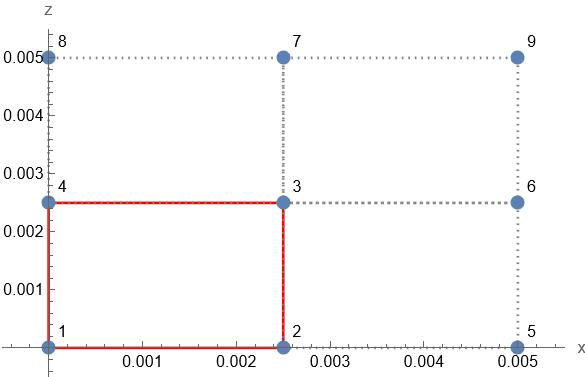
\includegraphics[width=0.7\textwidth, height=0.5\textwidth]{left-bottom-el.jpg}}
	\caption{Нижний левый конечный элемент на сетке 2 на 2 элементов}
	\label{left-bottom-el}
\end{figure}

Далее в цикле вычисляем все оставшиеся конечные элементы в этом ряду, на выбранной сетке он всего один. Поскольку новых узлов в сетке будет всего два, то необходимо будет использовать те же переменные для обозначения уже используемых узлов сетки. Как раз для этого и было сохранено значение индексов крайне правых элементов. Для осуществления слияния двух узлов разных конченых элементов уравнения для этих узлов складываются. В случае, если общие узлы оказываются граничными, то в сложение уравнений смысла не имеет - они и так отвечают граничным условиям. Добавляем в массив индексов верхних элементов новую пару узлов и сохраняем новые крайние правые узлы аналогично прошлому этапу. Аналогично с прошлым этапом учитываем граничные условия
\begin{figure}[!htbp]
	\center{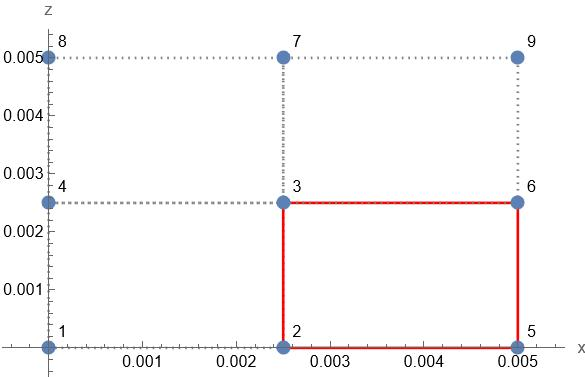
\includegraphics[width=0.7\textwidth, height=0.5\textwidth]{right-bottom-el.jpg}}
	\caption{Нижний правый конечный элемент на сетке 2 на 2 элементов}
	\label{right-bottom-el}
\end{figure}
\newpage
После этого переходим к вычислению конечных элементов выше по оси $z$.  Для этого будет использоваться цикл по вертикальной оси $z$. В рассматриваемом случае в этом цикле будет всего один ряд элементов, лежащих между 0.003 и 0.005 по оси $z$.
Рассмотрим вычисление элемента с узлами \{4,~3,~7,~8\}. Для него большая часть действий аналогично, не будем их повторять. Главной отличительной чертой алгоритма относительно прошлых конечных элементов будет использования массива индексов верхних узлов, который был заполнен на ранних этапах. Он нужен добавления в систему решения общих нижних узлов элементов - \{4,~3\}. Добавление происходит путем складывания имеющегося уравнения в системе с новым уравнением для вычисляемого узла. После все вычислений мы как и ранее сохраняем значение крайне правых узлов и обновляем индекс для крайне верхних узлов в массиве. Стоит заметить, что массив индексов крайне верхних узлов имеет размерность равную числу горизонтальных элементов сетки, то есть размерность 2 для рассматриваемого случае. В нем хранятся только актуальные для вычисления индексы.
\begin{figure}[!htbp]
	\center{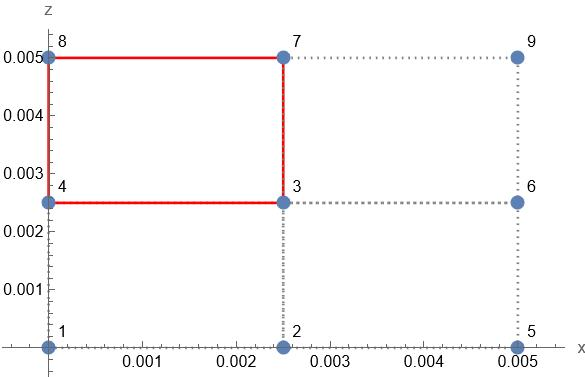
\includegraphics[width=0.7\textwidth, height=0.5\textwidth]{left-top-el.jpg}}
	\caption{Верхний левый конечный элемент на сетке 2 на 2 элементов}
	\label{left-top-el}
\end{figure}
\newpage
Для получения последующих уравнений для узлов конченых элементов используется цикл по оси $x$. Каких-то новых приемов для его вычисления не используется, расчет ведется аналогично с прошлыми элементами. В рассматриваемом случае такой элемент всего один.
\begin{figure}[!htbp]
	\center{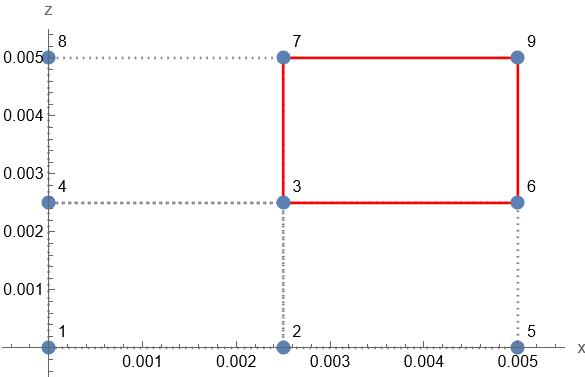
\includegraphics[width=0.7\textwidth, height=0.5\textwidth]{right-top-el.jpg}}
	\caption{Верхний правый конечный элемент на сетке 2 на 2 элементов}
	\label{right-top-el}
\end{figure}

Итого получаем систему линейных алгебраических уравнений, которая позволит получить нам давления в каждом из узлов сетки. Решаем систему с помощью встроенной в Wolfram Mathematica функции Solve и получаем решение задачи -- набор значений давлений в заданных узлах сетки.

\subsection{Верификация программы на основе обратной подстановки}
В качестве первого способа проверки вначале зададим функцию решения, вычислим для нее правую часть и затем подставим полученную правую часть в нашу программу. Важно чтобы выбранная нами функция удовлетворяла граничным условиям. Будем задавать функции с нулевыми граничными условиями. После подстановки правой части в программу будет возможно сравнить полученное решение со значениями функции заданной изначально.

В качестве первой проверочной функции рассмотрим
\begin{equation}
	f(x, z) = -2 \frac{\pi }{0.005} \sin{\left(\frac{\pi z}{0.005}\right)} x \left(x - 0.005\right)
	\label{check_func_1}
\end{equation}
Построим график функции~\eqref{check_func_1}
\begin{figure}[!htbp]
	\center{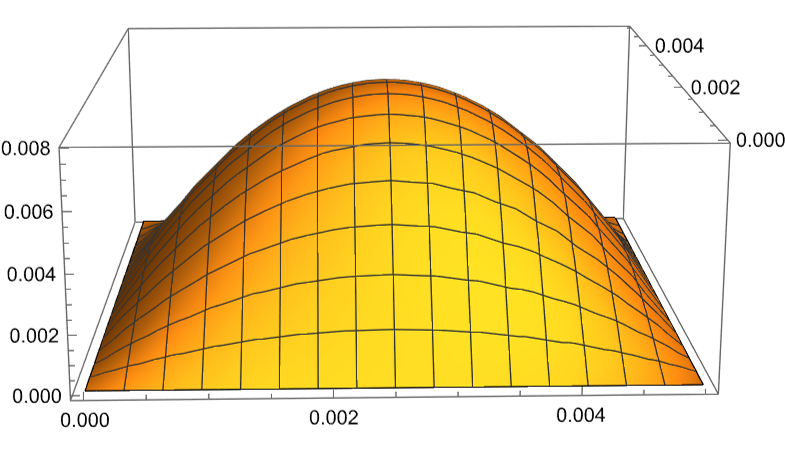
\includegraphics[width=0.9\textwidth, height=0.7\textwidth]{check_func_1.png}}
	\caption{Первая проверочная функция~\eqref{check_func_1}}
	\label{check_func_1_pic}
\end{figure}

\noindent Далее вычислим правую часть подставив~\eqref{check_func_1} в уравнение
\begin{equation*}
	F = \frac{\partial^2 f}{x^2} + \frac{\partial^2 f}{\partial z}
\end{equation*}
Полученную правую часть подставим в программу и будем искать искомую функцию $f$.

\begin{table}[!htbp]
	\begin{tabular}{|l|l|l|}
		\hline
		\multicolumn{1}{|c|}{Размерность сетки} & \multicolumn{1}{c|}{Разность, Па} & Погрешность, \% \\ \hline
		5 на 5                                  & 0.0002                              & 3.3            \\ \hline
		10 на 10                                & 0.0001                              & 0.8            \\ \hline
		20 на 20                                & 0.0000                              & 0.2            \\ \hline
	\end{tabular}
\end{table}

\noindent Поскольку форма функции весьма простая, то достаточно 10 элементов, чтобы получить решение с погрешность ниже одного процента.

Таким образом выглядит график полученного решения уравнения Рейнольдса на стеке 20 на 20. Визуальные отличия от искомого графика найти сложно.
\begin{figure}[!htbp]
	\center{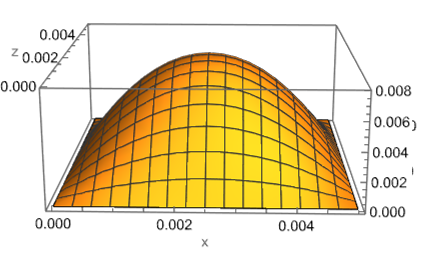
\includegraphics[width=0.7\textwidth, height=0.5\textwidth]{res_check_func_1.png}}
	\caption{Результат вычислений для проверочной функции~\eqref{check_func_1} на сетке 20 на 20}
	\label{res_check_func_1}
\end{figure}


Первая функция~\eqref{check_func_1} имеет простую форму, поэтому проблем с ее вычислением не ожидалось. Подберем более сложную функцию. В качестве второй проверочной функции рассмотрим
\begin{equation}
	f(x, z) = -2 \frac{\pi z}{0.005} \sin{\frac{2 \pi z}{0.005}} \sin{\frac{4 \pi x}{0.005}}
	\label{check_func_2}
\end{equation}

Построим график функции~\eqref{check_func_2}
\begin{figure}[!htbp]
	\center{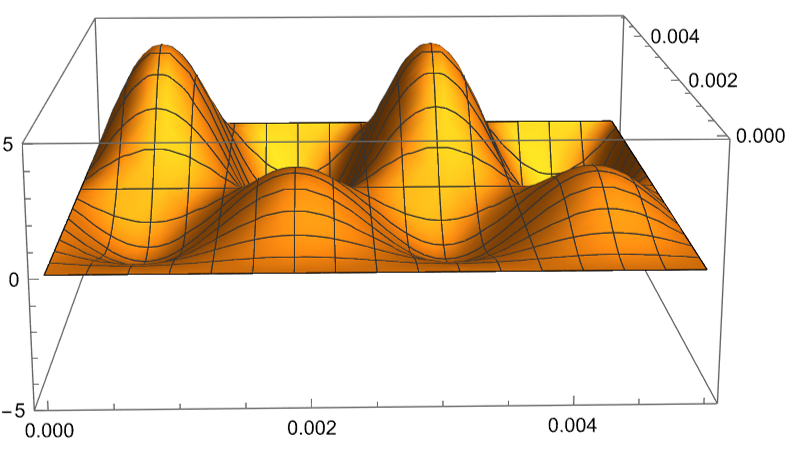
\includegraphics[width=0.65\textwidth, height=0.45\textwidth]{check_func_2.png}}
	\caption{Вторая проверочная функция~\eqref{check_func_2}}
	\label{check_func_2_pic}
\end{figure}

Правая часть вычисляется аналогичным образом с первой проверкой, подставив~\eqref{check_func_2} в уравнение
\begin{equation*}
	F = \frac{\partial^2 f}{x^2} + \frac{\partial^2 f}{\partial z^2}
\end{equation*} 

Посчитаем разность вычисленных значений с искомым и погрешность. Погрешность была вычислена по формуле $\underset{i}{\max} | \frac{{x_t}_i - {x_{node}}_i}{{x_t}_i} |$, где ${x_t}_i$ -- значение в узле $i$, полученное из искомой функции, а ${x_{node}}_i$ -- значение в узле $i$, полученное в программе. Максимум вычисляется по всем узловым элементам.

\begin{table}[!htbp]
	\begin{tabular}{|l|l|l|}
		\hline
		\multicolumn{1}{|c|}{Размерность сетки} & \multicolumn{1}{c|}{Разность, Па} & Погрешность, \% \\ \hline
		5 на 5                                  & 0.969                              & 21.31            \\ \hline
		10 на 10                                & 0.260                              & 5.7            \\ \hline
		20 на 20                                & 0.065                              & 1.4            \\ \hline
	\end{tabular}
\end{table}

Так выглядит результат работы программы для сетки 20 на 20 элементов.
\begin{figure}[!htbp]
	\center{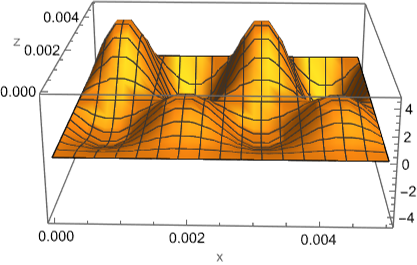
\includegraphics[width=0.6\textwidth, height=0.4\textwidth]{res_check_func_2.png}}
	\caption{Результат вычислений для проверочной функции~\eqref{check_func_2} на сетке 20 на 20}
	\label{res_check_func_2}
\end{figure}


Итого можно делать вывод, что на приведенных примерах программа считает верно, погрешность сокращается с увеличением числа элементов на сетке. Из двух проверок можно видеть, что для первой более простой по форме функции достаточно 10 элементов для получения небольшой погрешности, тогда как для более сложной второй функции нужно не мена сетка 20 элементов.



\subsection{Верификация программы сравнением с Wolfram Mathematica}

В качестве еще одной проверки воспользуемся пакетом компьютерной алгебры Wolfram Mathematica.
Решим уравнение Рейнольдса для $h(x) = -0.1x + 0.001$ и постоянного давления на границе $100000$ Па с помощью функции NDSolve.

\begin{figure}[!htbp]
	\center{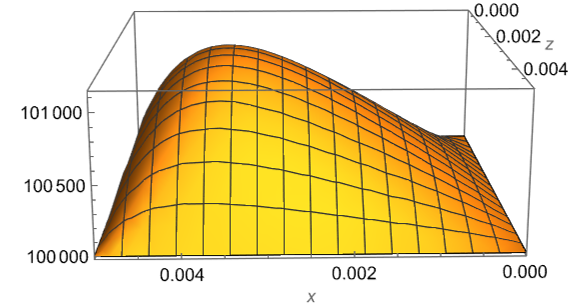
\includegraphics[width=0.7\textwidth, height=0.5\textwidth]{w_sol.png}}
	\caption{График решения, полученного с помощью Wolfram Mathematica}
	\label{w_sol}
\end{figure}

Сравним решения полученные с помощью собственной реализацией с решением Wolfram Mathematica.

\begin{table}[!htbp]
	\begin{tabular}{|l|l|l|}
		\hline
		\multicolumn{1}{|c|}{Размерность сетки} & \multicolumn{1}{c|}{Разность, Па} & Погрешность, \% \\ \hline
		5 на 5                                  & 1511	                              & 1.69            \\ \hline
		10 на 10                                & 1211                              & 1.19            \\ \hline
		20 на 20                                & 978                              & 0.96            \\ \hline
	\end{tabular}
\end{table}

Можно заметить, что даже на сетке 5 на 5 получаем близкий к численному решению Wolfram Mathematica. Такие результаты говорят о том, что созданная реализация МКЭ в данном примере выдает верный результат

Верификация работы программы была произведена двумя способами, таким образом можно судить о верности работы программы.

\subsection{Результаты моделирования}

Для демонстрации результатов рассмотрим различные функции зазора $h(x)$.  Расчеты будем проводить на сетке 10 на 10 со стандартными параметрами указанными в постановке задачи~\eqref{reinolts-task}.

В начале вычислим давление для постоянного зазора. Наблюдается симметрия по оси $x$, это верно, поскольку в уравнении Рейнольдса~\eqref{reinolts-task} правая часть будем нулевой из-за отсутствия переменной $x$ в функции зазора $h = 0.001$. Граничные условия соблюдаются. Можно сказать, что для постоянного зазора решается задача Лапласа.
\begin{figure}[!htbp]
	\center{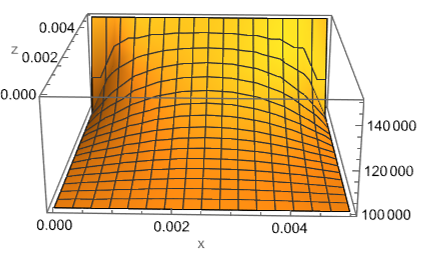
\includegraphics[width=0.7\textwidth, height=0.5\textwidth]{res_static.png}}
	\caption{График решения уравнения Рейнольдса для $h = 0.001$ м}
	\label{res_static}
\end{figure}

Затем получим график для увеличивающегося зазора. Наблюдается сдвиг по оси $x$ влево по сравнению с постоянным зазором. Это как раз и вызвано изменением в правой части уравнения Рейнольдса
\begin{figure}[!htbp]
	\center{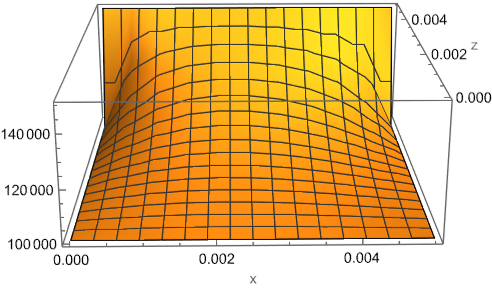
\includegraphics[width=0.7\textwidth, height=0.5\textwidth]{res_pos.png}}
	\caption{решения для $h = 0.001$ и $h = 0.15 x + 0.001$ м}
	\label{res_pos}
\end{figure}

Посмотрим подробнее на отличия растущего зазора и постоянного подробнее поточечно. Заметим, что левая часть точек чуть выше для графика решения уравнения Рейнольдса с  $h(x) = 0.15x + 0.001$, а правая напротив для графика решения уравнения Рейнольдса с $h(x) = 0.001$.

\begin{figure}[!htbp]
	\center{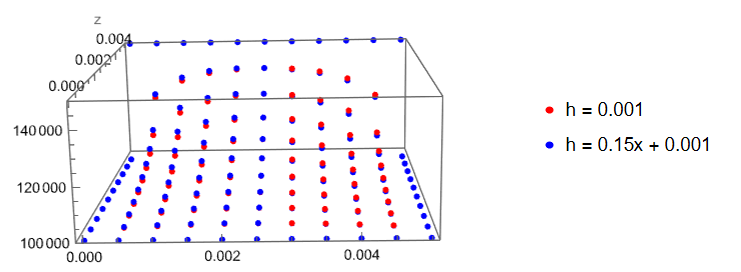
\includegraphics[width=\textwidth, height=0.45\textwidth]{pos_res_diff.png}}
	\caption{График решения уравнения Рейнольдса для $h = 0.15 x + 0.001$ м}
	\label{pos_res_diff}
\end{figure}


Далее аналогично рассмотрим зазор с отрицательным коэффициентом перед $x$. Так выглядит давление на пластину для уменьшающегося зазора. Наблюдается сдвиг по оси $x$ вправо по сравнению с постоянным зазором.

\begin{figure}[!htbp]
	\center{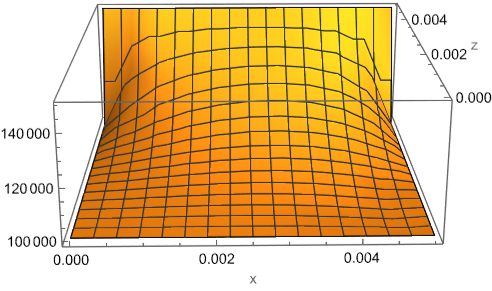
\includegraphics[width=0.6\textwidth, height=0.4\textwidth]{res_neg.png}}
	\caption{График решения уравнения Рейнольдса для $h = -0.15 x + 0.001$ м}
	\label{res_neg}
\end{figure}

Посмотрим подробнее на отличия уменьшающегося зазора и постоянного подробнее поточечно. Заметим, что правая часть точек чуть выше для графика решения уравнения Рейнольдса с  $h(x) = -0.15x + 0.001$, а левая напротив для графика решения уравнения Рейнольдса с $h(x) = 0.001$.

Получаем, что изменение знака <<зеркально>> меняет решение относительно оси $z$, что принципиально сходится с логикой результатов.

\begin{figure}[!htbp]
	\center{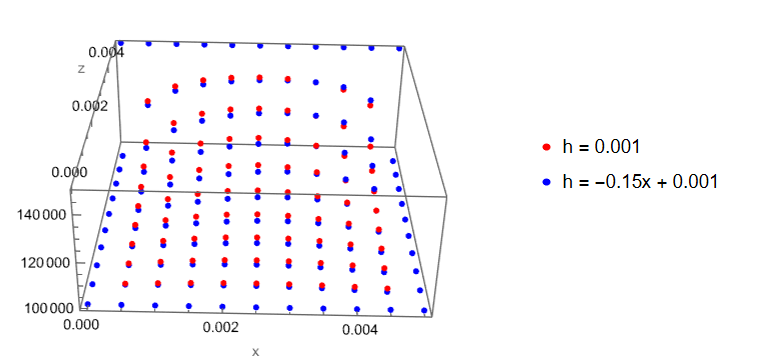
\includegraphics[width=0.9\textwidth, height=0.4\textwidth]{neg_res_diff.png}}
	\caption{Сравнение решения для $h = 0.001$ и $h = -0.15 x + 0.001$ м}
	\label{neg_res_diff}
\end{figure}

Чтобы более наглядно увидеть отличия которые вызывает знак перед коэффициентом у $x$ построим графики с одинаковыми граничными условиями на всех гранях равными $100000$ Па. Так мы получим явно вырожденную яму или пик -- в зависимости от знака коэффициента перед $x$ в функции зазора $h(x)$.

При отрицательном коэффициенте видим провал
\begin{figure}[!htbp]
	\center{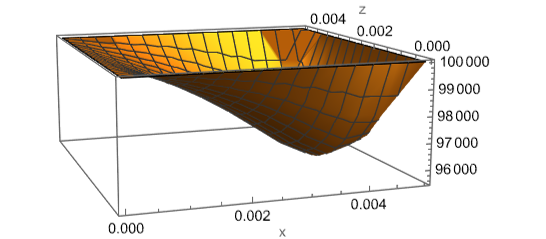
\includegraphics[width=0.7\textwidth, height=0.5\textwidth]{zero_neg.png}}
	\caption{График для $h = -0.15 x + 0.001$ м с одинаковыми ГУ}
	\label{zero_neg}
\end{figure}
При положительном коэффициенте наблюдаем пик
\begin{figure}[!htbp]
	\center{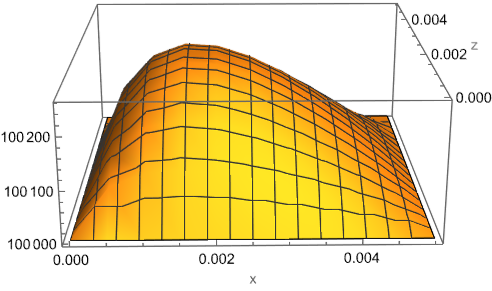
\includegraphics[width=0.7\textwidth, height=0.5\textwidth]{zero_pos.png}}
	\caption{График для $h = 0.15 x + 0.001$ м с одинаковыми ГУ}
	\label{zero_pos}
\end{figure}

Подводя итог первой главы, можно сказать, что была получена программа для решения уравнения Рейнольдса методом конечных элементов, проведена верификация верности ее работы двумя методами: подстановкой правой части и сравнением с функцией NSolve Wolfram Mathematica. Произведен ряд расчетов с ее помощью: для различного наклона зазора, равными и различными граничными условиями, результаты были сравнены между собой.

\section{Аэроупругая модель}
Имея рабочую программу по решению уравнения Рейнольдса, попробуем найти ей практическое применение и встроить ее в динамическую систему. Для ее получения можно дополнить имеющуюся модель пружиной, ограничивающей движение пластину сверху. Закрепим пружину по центру пластины в точке $\{0.0025, 0.0025\}$. Такая система имеет две степени свободы. На пружину также будет действовать внешнее давление $p_{ext} = 100000$ Па.

\begin{figure}[!htbp]
	\center{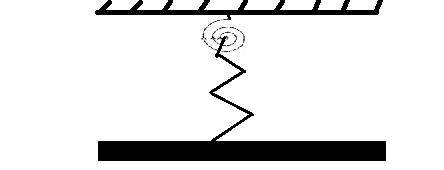
\includegraphics[width=0.7\textwidth, height=0.5\textwidth]{pruzina.png}}
	\caption{Схема модели пластины с пружиной}
	\label{pruzina}
\end{figure}


Необходимо связать изменения положения пластины и сжатия и растяжение пружины. Для этого необходимо записать уравнения Лагранжа. Они были разработаны французским математиком и астрономом Жозефом Луи Лагранжем в конце XVIII века. Идея уравнений Лагранжа второго рода заключается в том, что для описания движения системы достаточно знать ее кинетическую энергию и потенциальную энергию, а также уравнения, описывающие связи между различными частями системы. Эти уравнения выражаются в виде дифференциальных уравнений второго порядка, которые обеспечивают полное описание динамики системы. Поскольку имеем две степени свободы, то можно ограничиться двумя уравнениями Лагранжа.

Для записи уравнений Лагранжа обратимся к источнику~\cite{itmo} и зададим вертикальную координату l угловую $\psi$.
\begin{figure}[!htbp]
	\center{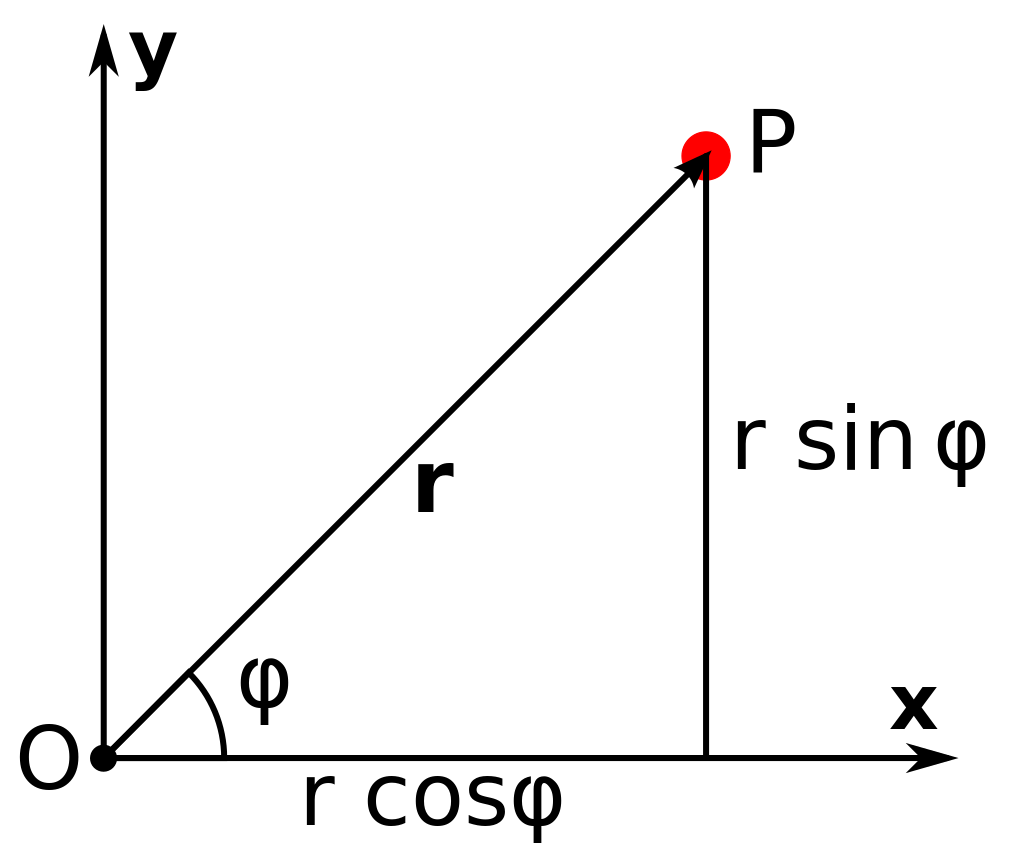
\includegraphics[width=0.7\textwidth, height=0.5\textwidth]{Polar_coordinate_components.png}}
	\caption{Полярная система координат}
	\label{Polar_coordinate_components}
\end{figure}

Тогда уравнения Лагранжа будут иметь вид~\cite{feodosiev}
\begin{equation}
	\begin{cases*}
	\frac{d}{dt} \left(\frac{\partial L}{\partial \dot{l}} \right) - \frac{\partial L}{\partial l} = F, \\
	\frac{d}{dt} \left(\frac{\partial L}{\partial \dot{\psi}} \right) - \frac{\partial L}{\partial \psi} = M,
	\end{cases*}
\label{lagrange}
\end{equation}
$F$ --- сила, $M$ --- момент. $L =  T - P$, где $T$ --- кинетическая энергия, а $P$ --- потенциальная.

\noindent Определим значения потенциальной силы
\begin{equation*}
	T = \frac{m \dot{l^2}}{2} + \frac{J \dot{\psi^2}}{2},
\end{equation*}
где $J = \frac{length^4}{12}$ --- момент инерции квадрата.

\noindent Определим значения потенциальной силы
\begin{equation*}
	P = \frac{k {l^2}}{2} +\frac{c {\psi^2}}{2},
\end{equation*}
где $k$ --- коэффициент жёсткости пружины на деформирование по $l$,  $c$ --- коэффициент жёсткости пружины на деформирование по $\psi$.

Функция $L$ будет иметь вид
\begin{equation*}
	L = \frac{m \dot{l^2}}{2} + \frac{J \dot{\psi^2}}{2} - \frac{k {l^2}}{2} +\frac{c {\psi^2}}{2}
\end{equation*}

После подстановки в исходную систему~\eqref{lagrange} получим
\begin{equation*}
	\begin{cases*}
		m \ddot{l} + k l = F, \\
		J \ddot{\psi} + c \psi = M,
	\end{cases*}
\end{equation*}
Для демпфирования добавим $\varepsilon \dot{l}$, где $\varepsilon$ --- постоянный коэффициент.
\begin{equation}
	\begin{cases*}
		m \ddot{l} + k l + \varepsilon \dot{l} = F, \\
		J \ddot{\psi} + c \psi = M,
	\end{cases*}
	\label{lagrange_fin}
\end{equation}

\subsection{Получение равновесного положения системы}

Первым этапом получения равновесного положения будет вычисление координат пластины, решая уравнение Рейнольдса с помощью ранее созданной программы. Начальный зазор $h(x) = 0.1 x + 0.0005$.
Далее поскольку ищем положение равновесия производные по времени в системе~\eqref{lagrange_fin} можно обнулить
\begin{equation}
	\begin{cases*}
		k l = F, \\
		c \psi = M,
	\end{cases*}
\label{temp_lagr}
\end{equation}
Определим силу $F$ и момент $M$ из полученного ранее давления. Для этого потребуется вычислить интегралы по площади конечного элемента. Обозначим $\hat{p_i} = p_i - p_{ext}$, где $i = 1..4$, $p_{ext} = 100000$ Па --- внешнее давление на пластину. Составим интегралы для силы и момента
\begin{equation*}
	F_i = \int_{S_i} { \left( N_1 \hat{p_1} + N_2 \hat{p_2} + N_3 \hat{p_3} + N_4 \hat{p_4} \right)  dx dz}
\end{equation*}
\begin{equation*}
	M_i = \int_{S_i} { \left( N_1 \hat{p_1} + N_2 \hat{p_2} + N_3 \hat{p_3} + N_4 \hat{p_4} \right) (x - 0.0025)  dx dz}
\end{equation*}
Вычислив их, можно получить значения $l$ и $\psi$ из~\eqref{temp_lagr}. Коэффициенты $k$ и $c$ сложно определить экспериментально, поэтому они были подобраны так, чтобы изменение зазора в достаточной степени влияло на положение пружины.

\begin{figure}[!htbp]
	\center{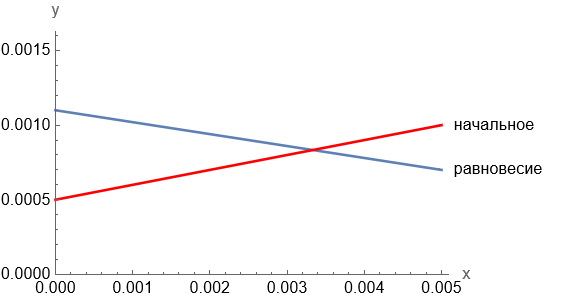
\includegraphics[width=\textwidth, height=0.5\textwidth]{part_2-zazor.png}}
	\caption{График для начального зазора $h(x) = 0.1 x + 0.0005$ и зазора в положении равновесия $h(x) = -0.08 x + 0.0011$}
	\label{part_2-zazor}
\end{figure}

После получения  $l$ и $\psi$ можно определить новый вид функции зазора $h(x) = x \tg{\psi} + l$. Далее снова переходим к решению уравнения Рейнольдса и процесс повторяется по кругу до тех пор пока функция  $h(x) = x \tg{\psi} + l$ перестанет изменяться.
За отсутствие изменений примем отсутствие изменений коэффициента и свободного члена до 5 знака после запятой. 
Получить равновесное значения $h(x)$ удалось за 4 повторения, $h(x) = -0.08 x + 0.0011$. 
Решение уравнения Рейнольдса для такого зазора изображено на~рис.\ref{part_2-zazor}.

\noindent Итак, было получено некое положение равновесия динамической системы. Далее следует убедиться в устойчивости данного положения пластины.


\subsection{Проверка устойчивости системы}
Полученное положение равновесия может быть не устойчиво. Простейшим примером такого положения может быть математический маятник в самом верхнем вертикальном положении. При придании маятнику в таком положении малейшего смещения он сразу же покинет положение устойчивости и начнет колебания. Поэтому для проверки устойчивости нужно изменять значения $l$ и $\psi$ на 1-2\% в большую и меньшую сторону.  Таким образом  можно построить аппроксимацию $F$ и $M$ из системы~\eqref{temp_lagr}. Аппроксимация полиномиальная вида $F = F_0 + d_1 \Delta{l} + d_2 \Delta{\psi}$, $M = M_0 + u_1 \Delta{l} + u_2 \Delta{\psi}$.
В искомой системе~\eqref{lagrange_fin} $l$ и $\psi$ заменяются на $l_0 + \Delta{l}$ и $\psi_0 + \Delta{\psi}$ соответственно. $l_0$, $\psi_0$ --- значения координат в равновесии системы. После подстановки момента и силы, а также замены $l$ и $\psi$ коэффициенты отвечающие за равновесность состояния сокращаются. После этого следует произвести еще две замены
\begin{equation*}
	\Delta{l} = L \exp{w t}
\end{equation*}
\begin{equation*}
	\Delta{\psi} = \Psi \exp{w t}
\end{equation*}
$w$ имеет физический смысл частоты колебаний, считаем, что частота колебания по обоим осям одинаковая. $L$ и $\Psi$ --- амплитуды колебаний.
После проведения всех замен и группировки слагаемых получим систему
\begin{equation*}
		\begin{cases*}
			\left( m \omega^2 - d_1 - \varepsilon \omega + k \right) L - d_2 \Psi = 0, \\
			\left( J \omega^2 - u_2 = c \right) \Psi - u_1 L = 0.
		\end{cases*}
\end{equation*}
Если определитель будет не равен нулю, то решение системы будет только тривиальное. При определителе неравным нулю получим бесконечно много решений пропорциональных нагрузке. Из условия равенства нулю определителя получаем
\begin{equation*}
			m J w^4 - \varepsilon J w^3 + \left( \left(c - u_2 \right) m + \left(k - d_1 \right)J \right) w^2 + \left(u_2 - c\right) \varepsilon w + 
\end{equation*}
\begin{equation*}
	+ d_1 \left( u_w - c \right) - k \left( u_2 - c \right) - d_1 u_1 = 0
\end{equation*}
\noindent Теперь можно определить устойчивость равновесия по критерию Рауса-Гурвица. 

\textbf{Критерий Рауса—Гурвица.}
Пусть имеем линейное дифференциальное уравнение с постоянными вещественными коэффициентами:
\begin{equation*}
	a_0 y^{(n)} + a_1 y^{(n - 1)} + ... + a_n y  = 0, (a_0, a_1, ..., a_n = const, a_0 > 0).
\end{equation*}
Нулевое решение $y = 0$ уравнения асимптотически устойчиво, если все корни характеристического уравнения 
\begin{equation*}
	а(\lambda) = a_0 \lambda^n + a_1 \lambda^{n - 1} + ... + a_n = 0.
\end{equation*}
имеют отрицательные вещественные части. Для того чтобы это выполнялось необходимо и достаточно, чтобы были положительными все главные диагональные миноры матрицы Гурвица.

Запишем коэффициенты $a_i$
	\begin{equation*} 
	\begin{cases}
		a_4 = m J, \\
		a_3 = - \varepsilon J, \\
		a_2 = \left(c - u_2 \right) m + \left(k - d_1 \right)J, \\
		a_1 = \left(u_2 - c\right) \varepsilon, \\
		a_0 = d_1 \left( u_2 - c \right) - k \left( u_2 - c \right) - d_2 u_1.
	\end{cases}
\end{equation*}
Для устойчивости должно выполняться 
	\begin{equation*} 
	\begin{cases}
		\Delta_1 = a_1 >  0, \\
		\Delta_2 = a_1 a_2 - a_0 a_3 > 0, \\
		\Delta_3 = \begin{vmatrix*}
			a_1 & a_0 & 0 \\
			a_3 & a_2 & a_1 \\
			0 & a_4 & a_3 
		\end{vmatrix*} > 0.
	\end{cases}
\end{equation*}
После вычислений получим 
\begin{equation*} 
	\begin{cases}
		\Delta_1 = 18.05 > 0, \\
		\Delta_2 = 0.000064 > 0, \\
		\Delta_3 = 2.7 \cdot 10^{-14} > 0
	\end{cases}
\end{equation*}
Поскольку все определители больше нуля, то можно говорить о том, что положение равновесия устойчивое.

Таким образом мы показали устойчивость полученного положения равновесия. Функция зазора $h(x) = -0.08 x + 0.0011$ соответствует устойчивому положению равновесия, что было доказано по определению асимптотической устойчивости.

\subsection{Особенности реализации}
В численной реализации описанного алгоритма есть некоторые особенности, на которые стоит описать отдельно.

Во-первых, это связь программы решения МКЭ уравнения Рейнольдса и вычисления новой функции зазора $h(x)$ из уравнений Лагранжа. Для вычисления силы и момента, фигурирующих в системе~\eqref{temp_lagr} требуется сохранить все значения индексов узлов поэлементно, а также смещение для перехода из глобальной системы координат в локальную. Для этого на каждом шаге вычисления необходимо определять индекс элемента массива, которые соответствует этому узлу. В этом помогают описанные ранее массивы последних правых индексов и последних верхних.

После вычисления моментов и сил для каждого элемента они складываются между собой для получения искомых $F$ и $M$ из системы~\eqref{temp_lagr}.

Для получения функций аппроксимации силы $F$ и момента $M$ использовалась функция Wolfram Mathematica FindFit. Функция аппроксимации ищется в форме многочлена первого порядка со свободным членом.




\newpage
%\section-{\large{ЗАКЛЮЧЕНИЕ}}
\section-{\large{Заключение}}
В работе представлена модель решения уравнения Рейнольдса для установившегося течения в газовом смазочном слое построенная с помощью метода конечных элементов. По итогам работы можно выделить следующие моменты:
	\begin{enumerate}	
		\item Показано, что исследование устойчивости положения равновесия сегментов надроторного кольца в потоке жидкости можно выполнить на основе инженерного подхода, объединяющего модель Рейнольдса для течения жидкой смазки и модель колебательной системы с двумя степенями свободы.
		\item Показано возникновение подъемного гидродинамического клина в сужающемся по окружности зазоре, а также области разряжения в зазоре с расширением. Эти результаты согласуются с экспериментально наблюдаемой картиной течения в гидродинамических подшипниках и уплотнениях.
		\item Построенная математическая модель может быть использована на этапе предварительного проектирования конструкции.
	\end{enumerate}

\newpage


%\section-{\large{СПИСОК ИСПОЛЬЗОВАННЫХ ИСТОЧНИКОВ}}
\section-{\large{Список использованных источников}}
\begin{thebibliography}{00}
\bibitem{petrov_smazka} Петров Н.П. Гидродинамическая теория смазки, М.: из-во академии наук СССР, 1948. --- 558~с.
\bibitem{slezkin_smazka} Слезкин Н.А. Динамика вязкой несжимаемой жидкости, М.: из-во техно-теоретической литературы, 1955. --- 521~с.
\bibitem{seligard} Селегринд Л. Примененение метода конечных элементов, М.: из-во МИР, 1979. --- 195~с.
\bibitem{seshu} Seshu P. Textbook of
Finite Element
Analysis, New Dehli: PHI Learning Private Limited, 2012. --- 340~с.
\bibitem{itmo} Григорьев А.Ю., Григорьев К.А., Малявко Д.П. Колебания
и виброактивность элементов машин: Учеб. пособие. СПб.: Университет ИТМО, 2016. --- 136~с.
\bibitem{sel-1}  Селиванов А.В., Дзева И.Ю., Многодисциплинарная математическая модель пальчикового уплотнения Уфа:, 2011 --- 17 c.
\bibitem{feodosiev} Феодосьев В.И. Сопротивление материалов: Учеб. для вузов. М.: Изд-во МГТУ им.
Н.Э. Баумана, 1999. – 592 с.
\bibitem{nasa} Steinetz B.M., Hendricks C.R. Overview of NASA Glenn Seal Development
Program. Nevada: NASA
Conference Publication, 2001 --- 493 с.

\end{thebibliography}

\newpage

%\section-{\large{ПРИЛОЖЕНИЕ А}}
\section-{\large{Приложение А}}

Результаты решения уравнения Рейнольдса МКЭ с постоянным зазором.
\begin{figure}[!htbp]
	\center{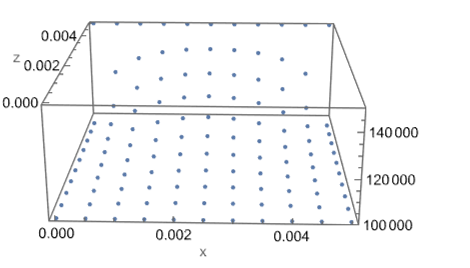
\includegraphics[width=0.5\textwidth, height=0.3\textwidth]{prilozh_const.png}}
	\label{prilozh_const}
\end{figure}

Результаты решения уравнения Рейнольдса МКЭ с увеличивающимся зазором.
\begin{figure}[!htbp]
	\center{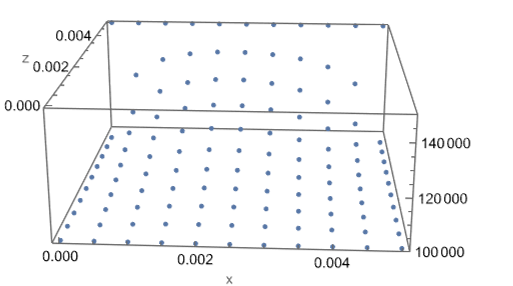
\includegraphics[width=0.5\textwidth, height=0.3\textwidth]{prilozh_pos.png}}
	\label{prilozh_pos}
\end{figure}

Результаты решения уравнения Рейнольдса МКЭ с уменьшающимся зазором.
\begin{figure}[!htbp]
	\center{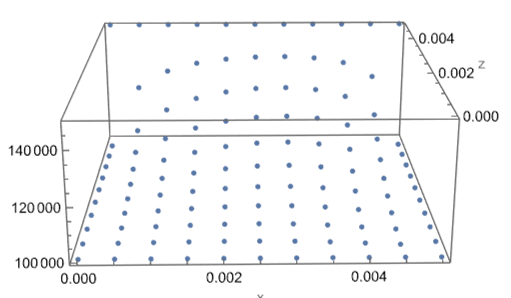
\includegraphics[width=0.5\textwidth, height=0.3\textwidth]{prilozh_neg.png}}
	\label{prilozh_neg}
\end{figure}

\end{document} 